% Document history:
%  1.0 - Original version by W. H. Bell
%  1.1 - Updated text
%
\documentclass[11pt]{scrartcl}
\usepackage{graphicx}
\usepackage{acronym}
%\usepackage{moreverb}
\usepackage{fancyhdr}
\usepackage{float}
\usepackage{listings}
\usepackage{color}
\usepackage{epstopdf}

\definecolor{LightGrey}{rgb}{0.93,0.93,0.93}

\lstset{basicstyle=\small,showstringspaces=false}
\lstset{language=C}
\lstset{backgroundcolor=\color{LightGrey}}
\lstset{postbreak=\space, breakindent=5pt, breaklines}
%\lstset{xleftmargin=5pt, xrightmargin=5pt}
%\lstset{framexleftmargin=5mm,frame=shadowbox,rulesepcolor=\color{LightGrey}}


\setlength{\parskip}{1.5ex\relax}

\setlength{\fboxsep}{2mm} \setlength{\fboxrule}{0.8pt}  %% default=0.4

% Problems with this function:
%    1. Breaks headings as they loose the \noindent
\newcommand{\funbox}[1]{\vbox{\vspace{0.2cm}\fbox{\large\texttt{#1}}\vspace{0.2cm}}}
\def\cpp{C$++$}
\def\main{\texttt{main()}}
\def\intmain{\texttt{int main()}}
\def\void{\texttt{void}}
\def\psc{Pseudocode}
\def\flo{Flowchart}
\def\fortran{FORTRAN}
\def\linux{Linux}

\floatstyle{plain}
\newfloat{program}{thp}{lop}
\floatname{program}{Listing}

\floatstyle{boxed} %ruled
\newfloat{pseudocode}{thp}{lop}
\floatname{pseudocode}{Pseudocode}

\begin{document}
\title{C programming for physicists}
\author{W. H. Bell}
\date{
\copyright 2015
}

\maketitle
\hrule
\vspace{0.2cm}
\begin{abstract}
The C programming language is introduced through a set of worked examples.  An introduction to programming in the \linux\ environment is given, together with design tools such as flowcharts and \psc.  Following the initial discussion of programming concepts, the majority of the ANSI C syntax and build in commands are demonstrated.  The course concludes with a more complicated example of histogramming data from a particle physics simulation.
\end{abstract}
\vspace{0.2cm}
\hrule

\clearpage
\newpage

\tableofcontents

\clearpage
\newpage

\pagestyle{fancy}

\section{Introduction}
\paragraph{Aims}
\begin{enumerate}
\item Learn to solve problems by implementing computer programming structures and designs suitable for use with any structured programming language.
\item Cover core aspects of the C programming language.
\item Introduce programming with a \linux\ platform. 
\end{enumerate}

\paragraph{Syllabus}
\begin{itemize}
  \item Problem analysis strategies
  \begin{itemize}
    \item Flowcharts
    \item \psc 
  \end{itemize}
  \item ANSI C
  \begin{itemize}
    \item Basic syntax and variable types
    \item Arrays, pointers and functions
    \item The C preprocessor
    \item Input/Output operations
    \item Structures and unions 
  \end{itemize}
  \item Introduction to programming on \linux
  \begin{itemize}
    \item The GNU C Compiler (\texttt{gcc})
    \item Building executables with \texttt{make} 
  \end{itemize}
\end{itemize}

Material taught within the syllabus is intended to be supplemented by
further reading. The recommended reference material for this course
is:
\begin{itemize}
\item ``The C Programming Language'', Brian W. Kernighan and Dennis M. Ritchie, Prentice-Hall, ISBN 0-13-110362-8
\end{itemize}
Further information on the GNU C compiler can be found at \cite{gcc}.

\subsection{Motivation}
Computers can be used for data acquisition, control, statistical analyses, building simulations, numerical methods and other generalised complex systems.  While many software packages have been written, it is often necessary to write or modify software to facilitate research or meet a goal within the workplace.  Those who are able to program are therefore in an excellent position to attack complex problems.

\subsection{Programming}
There are a great many different computer programming languages.  Thankfully, once the general process of programming has been understood it does not take a great deal of effort to apply similar strategies to other languages.  The C programming language was chosen for this course for several reasons: (i) the basic syntax is the same as \cpp\ and JAVA, (ii) its structured layout is similar to other common languages, (iii) the language is simple and therefore easily understood, (iv) C is used in many modern applications.

\subsection{Writing Programs} %HHH
Before a program is written it is important to know what is actually
needed.  For example a program that will be used for data acquisition
must be tailored to the specific hardware that will be used and
provide a user interface which contains all the needed functionality.
Failure to properly understand the requirements of a program  
may result in wasted time, redesigning or patching at a
later stage.  Some complicated languages such as \cpp\ are particularly
unforgiving in this respect.

Once the requirements have been listed the overall aims needed from a
program can be broken down into a series of pieces which can be easily
converted into a computer language.  During this course
\psc~\cite{pseudocodewiki} and Flowcharts~\cite{flowchartwiki}
will be used to assist with programming design.

Flowcharts provide a high level design tool which can also be used as
a form of documentation.  They promote a logical thought process by
following a set of construction rules.  It is however very time
consuming to design every corner of a program with them.  Flowcharts
should therefore be used either to describe the overall logic of a
program or particularly difficult to understand section of a program.

\psc\ is as the name suggests code which is not really code, but
is instead a way of describing a program.  Writing \psc\ provides
a quick way of breaking a problem down into component parts.  There is
however no fixed standard and it is therefore probably best to find a
way of writing \psc\ that feels comfortable to you.  \psc\
is more a design tool than a form of documentation although much of
what is written in \psc\ will often end up as comments within a
program.

In summary the process of writing a program can be summarised in 4
steps: (i)~Requirements, (ii)~Design, (iii)~Implementation, and 
(iv)~Documentation.  When writing a program it is a good idea to have
a log book and scrap paper handy to facilitate this process.

\subsection{Programming with Linux}
The example programs that are discussed in this guide can be downloaded from:
\begin{verbatim}
http://www.whbell.net/resources/PhysCIntro/
\end{verbatim}
Once the examples have been downloaded, they can be unpacked using the tar command:
\begin{verbatim}
]$ tar PhysCIntroSource-2015-06-21.tar.gz
\end{verbatim} %$
where \texttt{$]\$$} refers to the \linux\ prompt.  Each subdirectory contains source code and a \texttt{README.txt} file that describes how to build and run the associated example program.

When developing C it can be very helpful to use an editor that colours
text according to C syntax.  \texttt{xemacs} and \texttt{emacs} provide this
functionality.  Syntax highlighting in \texttt{xemacs} can be enabled by
clicking on \texttt{Options$\rightarrow$Syntax~Highlighting} at the
top of the editor window, and selecting \texttt{In~This~Buffer},
\texttt{Automatic}, \texttt{Force~Rehighlight~in~this~Buffer},
\texttt{Fonts} and \texttt{Colors}.  \texttt{xemacs} and
\texttt{emacs} also provide 
many other helpful features such as parenthesise checking and tab stops
positioning according to the syntax used.

%%%%%%%%%%%%%%%%%%%%%%%%%%%%%%%%%%%%%%%%%%%%%%%%%%%%%%%%%%%%%%%%%%%%%%%%%%%%

\section{Beginning to program with C}

\subsection{A first program}

Programming languages are commonly introduced by writing a program to
print a string to the standard output.  The standard output is the
terminal window or screen.  Therefore information printed to the
standard output will appear on the terminal window or screen.  Before
looking at the example program let us look at its design.
Figure~\ref{figure:flowchart_ex1} illustrates example 1 in \flo
form, \psc~\ref{pseudo:ex1} describes the program using
\psc and the C implementation of example 1 is given in
Listing~\ref{listing:ex1}.

\begin{figure}[h]
\begin{center}
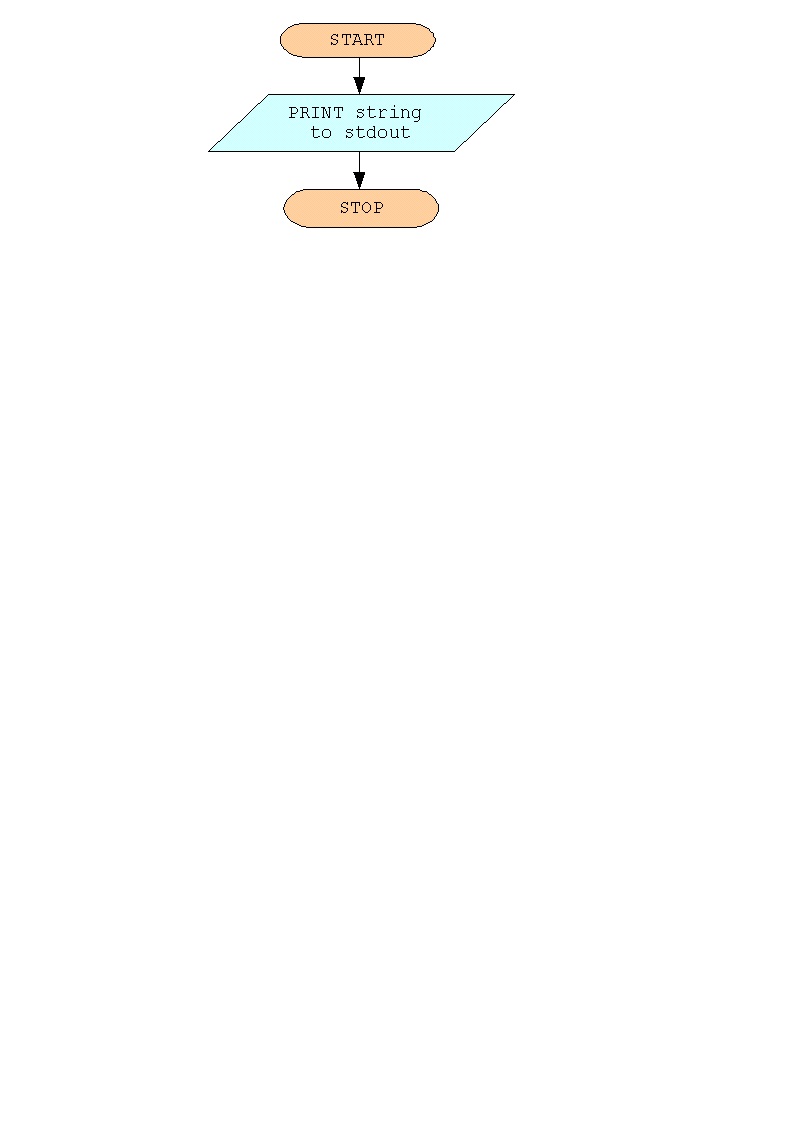
\includegraphics[height=3cm]{figures/ex1}
\caption{A flowchart describing example 1
\label{figure:flowchart_ex1}}
\end{center}
\end{figure}

\begin{pseudocode}[h]
\begin{verbatim}
main()
  Print a string
  Return 0 to the operating system
\end{verbatim}
\caption{Example 1 in pseudocode \label{pseudo:ex1}}
\end{pseudocode}

\begin{program}[H]
\begin{lstlisting}
/* W. H. Bell
** A very simple C program to print one line to the standard out
*/

#include <stdio.h>

int main() {
  printf ("In the beginning...\n");
  return 0;
}
\end{lstlisting}
\caption{The C implementation of Example 1 \label{listing:ex1}}
\end{program}

The execution of every program starts from a \main function.  From
this function other functions can be called.  The return type of \main
is given by the \texttt{int} prefix.  Within the \linux/UNIX
environment the operating system expects a program to return an exit
condition.  The value of the return statement from the \main\ function
is collected by the operating system and is available to a user to
query.  Following the execution of the program the return value can
be queried by typing
\begin{verbatim}
]$ echo $?
\end{verbatim}
where \texttt{$]\$$} is the LINUX prompt.

The contents of the \main\ function are delimited by the brackets
\texttt{\{ \}}, which represent a compound statement.  Inside this
compound statement there may be several statements each terminated by a
`\texttt{;}' character, together with other compound statements.  In
this example the \main function only contains two statements: one to
print a string to the standard output and one to return the exit value to
the operating system.  The first of these statements prints a string
to the screen by calling the standard output function
\texttt{printf}.  This string is terminated by the end of line character \texttt{$\backslash$n}.  At the top of the example, the
pre-declaration of the \texttt{printf} function is included by
including the header file \texttt{stdio.h}.  When this program
compiles the compiler reads the pre-declaration of \texttt{printf}
from the header file and leaves a call in the machine code to be
resolved at link time.  Above the \texttt{\#include} statement is a
comment.  Comments in C can be entered using
\texttt{/* */} to surround the comment area.\footnote{The use of
\texttt{//} comments is a non-ANSI feature and is therefore not
included in this course.}  When the compiler compiles the code it
ignores any text surrounded by \texttt{/* */}.

\clearpage
\newpage

\subsection{Loops, Conditional Statements and Functions}
Example 2 introduces functions, conditional statements and loops.
The example reads from the standard input and performs several
checks on integers and characters provided by the user.  (The standard
input refers to something typed into a terminal by either the keyboard
or by redirection.)  A \flo\ describing the \main\ function is
given in figure~\ref{figure:flowchart_ex2}.  A \psc\
implementation of this program is given in \psc~\ref{pseudo:ex2}.

\begin{figure}[h]
\begin{center}
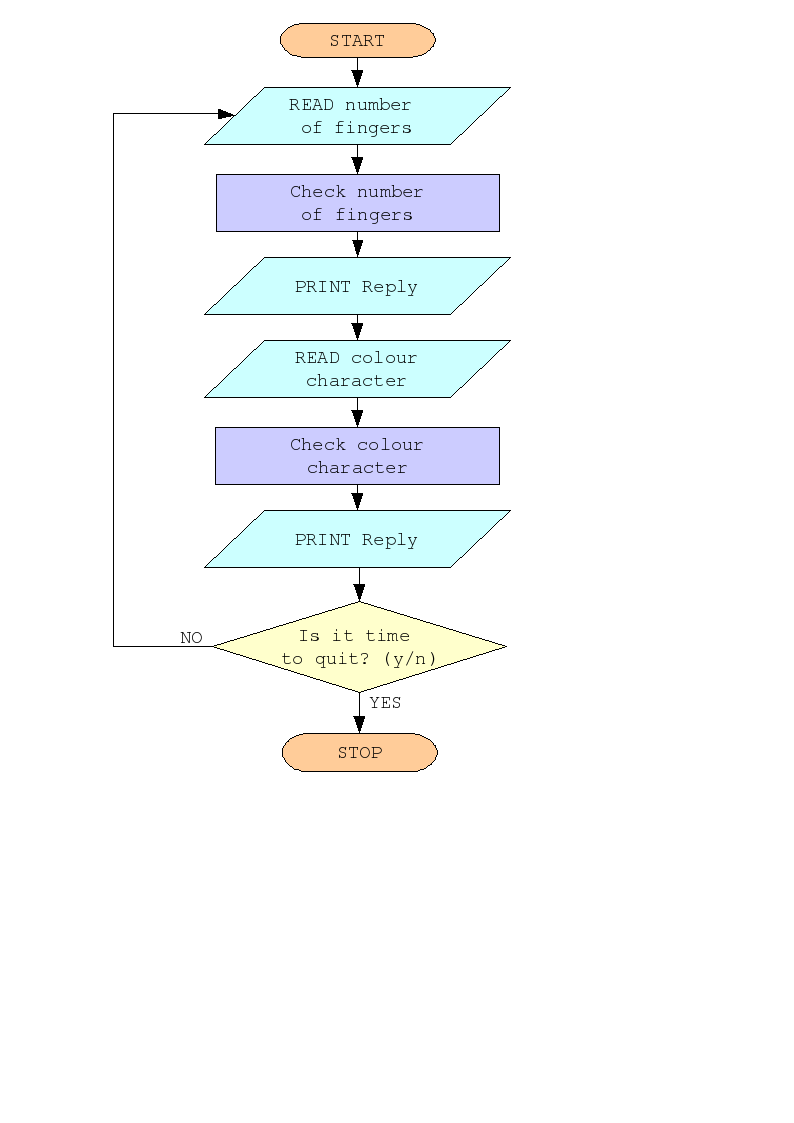
\includegraphics[height=11cm]{figures/ex2}
\caption{A flowchart describing the \main\ function of example 2
\label{figure:flowchart_ex2}}
\end{center}
\end{figure}

\begin{pseudocode}[h]
\begin{verbatim}
main()
  DO
    Check the number of fingers.
    Check the colour.
  WHILE not time to quit

numFingers()
  Print the question
  Read a number from the stdin
  Compare the number and return an answer

pickColour()
  Print the question.
  Read a character from the stdin.
  Compare the character and return an answer.

quitTime()
  Ask the user if it is time to quit (y/n)
  Collect a character from the stdin
  Compare this with y/Y and return 1 if its is time to quit
\end{verbatim}
\caption{Example 2 in pseudocode \label{pseudo:ex2}}
\end{pseudocode}

\paragraph{Functions}
The syntax of loops, conditional statements and functions are
demonstrated by example 2.  This example contains an \intmain function
as before.  Within the \main three functions are called:
\texttt{numFingers}, \texttt{pickColour}, and
\texttt{quitTime}.  Each function is pre-declared before the \main
function.  Each pre-declaration is a statement where the return type,
and input parameter types must be given.  The \void type simply means that
no input parameter or return value is expected.  All functions must be
either predeclared or declared before they are used.  There are three
pre-declaration statements before the \main function.
\begin{lstlisting}
void numFingers(void);
void pickColour(void);
bool quitTime(void);
\end{lstlisting}
The implementation of these functions is given after the \main
function.  Following the same syntax as the \main function the
implementation of each of these three functions has a return type, a
series of input types, and a compound statement enclosing the function
contents.  If any input parameters are present then their names must
be given.  These input variables are introduced with the values passed
into the function when the function is called.  If the implementation
is not given in either the code to be compiled or libraries to be
linked in a linker error will result.

It should be noted that while in this example the function
pre-declarations are given before the \main and the implementation
comes afterwards, the example would work just as well with the
implementation before the \main and no pre-declarations.  The use of
pre-declarations at this point is a lead-in to the usage of header
files which are later introduced in example 5.

\paragraph{Conditional Statements}
Common ways of writing conditional statements involve either
\texttt{if},~\texttt{if~else},~\texttt{else} or \texttt{switch}
statements.  There are other ways of constructing conditional
statements but these are not covered in this course.  Starting with
\texttt{if},~\texttt{if~else},~\texttt{else} statements, examples of
their syntax are given within the \texttt{numFingers} and \texttt{quitTime}
functions of example 2.  Each \texttt{if} statement is evaluated such
that when the contents of the logic associated with an \texttt{if} statement
inside the \texttt{()} brackets is true, then the code within the
following compound statement is executed.
\texttt{if},~\texttt{if~else},~\texttt{else} statements operate
sequentially such that each piece of logic is tested in turn.  If all
the logic tests fail then the statement following \texttt{else} is
executed.

In some cases where simple sorting is needed a \texttt{switch}
statement is a better choice than a long
\texttt{if},~\texttt{if~else}...~\texttt{else} statement.  An example
\texttt{switch} statement is given in the \texttt{pickColour} function
of example 2.  While faster than an
\texttt{if},~\texttt{if~else},~\texttt{else} statement in some cases a
\texttt{switch} statement is limited to simple cases and therefore the
logic allowed can be somewhat restrictive.

\paragraph{Loops}
Several types of loops are available to C programmers.  There are
\texttt{while}, \texttt{do~while} and \texttt{for} loops.  Each of
these loops continue to loop while a condition is true.  All the logic
available within an \texttt{if} conditional statement is also
available within these conditional tests.  Instances of these loop
types can be found within some of the examples within this course.
Within this section example 2 contains a \texttt{do~while} loop in its
\main function.  This loop continues while
the boolean evaluated within the \texttt{while(~);} is true.  This
remains true until the function \texttt{quitTime} returns a true.  The
\texttt{while} loop tests on NOT \texttt{quitTime} return value.

\subsection{Pointers and Arrays \label{section:pointersarrays}}

Many languages use pointers implicitly such as \fortran and Java.  In
C pointers are used explicitly.  This section introduces the concept
of a pointer and demonstrates two basic implementations.  The design
of the program is given in \flo form in
figure~\ref{figure:flowchart_ex3} and in \psc form in
\psc~\ref{pseudo:ex3}.

\begin{figure}[h]
\begin{center}
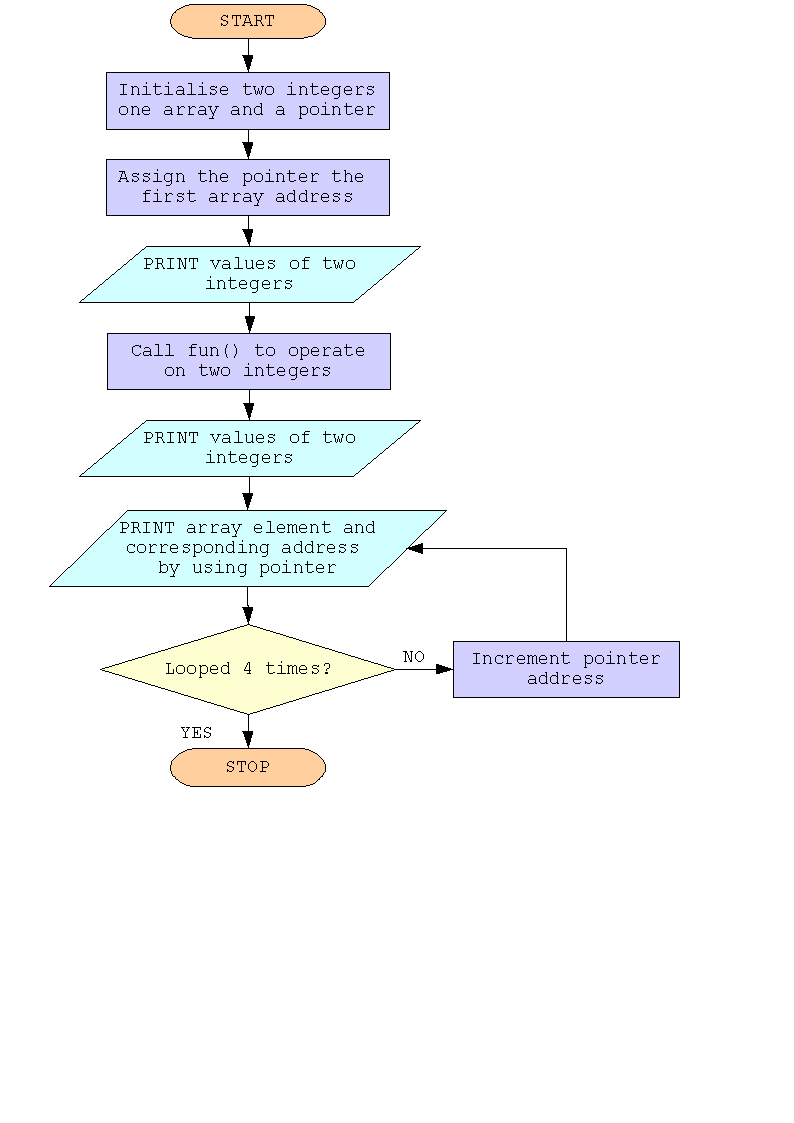
\includegraphics[height=11cm]{figures/ex3}
\caption{A flowchart describing the \main function of example 3
\label{figure:flowchart_ex3}}
\end{center}
\end{figure}

\begin{pseudocode}[h]
\begin{verbatim}
main()
  Initialise two np and p integers with 1.
  Initialise an array v with four elements.
  Initialise a pointer pv with the address of the first element of the
  array. 

  Print the values of the two integers np and p.
  CALL fun() with the value np and the address &p.
  Print the values of the two integers np and p.

  Iterate over the array indices using the pointer pv.
    Print the contents and address of each array element using pv.

fun(value and pointer)
  Assign a number to the local variable.
  Assign a number to the memory the pointer points to.
\end{verbatim}
\caption{Example 3 in pseudocode \label{pseudo:ex3}}
\end{pseudocode}

Pointers are called pointers because they point to a memory address.
A pointer can be used to access the memory address to which it points
or the value contained within the memory address.  The C
implementation of example 3 introduces pointers.  Looking at example 3
there are two distinct parts to the program: the call to the function
\texttt{fun} and the indexing of array \texttt{v[]}.

\paragraph{Functions and Pointers}
The function \texttt{fun} is declared as 
\begin{lstlisting}
void fun(int, int *);
\end{lstlisting}
with input parameter types \texttt{int} and \texttt{int *}.  The
second input parameter is a pointer.  When the function is called the
memory address of \texttt{p}, \texttt{\&p} is assigned to the pointer
declared in \texttt{fun}.  The importance of using a pointer in this
fashion can be seen from running the program.  After calling
\texttt{fun}, \texttt{np} contains the same value which it contained
before the function call, while the value contained in \texttt{p} is
the value assigned via the pointer in
\texttt{fun}.  Stepping through the program this can be explained.
Both \texttt{np} and \texttt{p} are initialised in the \main with the
value one.
\begin{lstlisting}
int np = 1, p = 1;
\end{lstlisting}
At the point of initialisation an \texttt{int} sized block of memory
is allocated to \texttt{np} and \texttt{p}.  Then the function
\texttt{fun} is called with the value of \texttt{np} (default in C) and the
address of \texttt{p}.  Within the function \texttt{fun} a new block
of memory is allocated for the local variable \texttt{np} distinct
from the variable contained in the \main function.  This memory is
given the value from the parameter \texttt{np} contained within
\main.  The value 2 is assigned to the local variable \texttt{np}
and as the function exits, the memory of the local variable \texttt{np}
is deleted.  Therefore the value is never set within the \main
function.  Unlike \texttt{np} the value of the variable \texttt{p}
declared within
the \main is set by using a pointer.  The pointer is initialised with the
memory address of the variable \texttt{p} contained within the \main
function.  Then the memory address pointed to by the pointer
\texttt{*p} is assigned the value 2.  Therefore when returning to the
\main function the value contained in the memory of \texttt{p} is
still 2.

\paragraph{Arrays and Pointers}
An array of type '\texttt{t}' is a series of memory blocks of size
according to the type.  Each element of the array behaves as a
separate variable of the given type of the array.  Array sizes are
determined at compile time and therefore must be declared somewhere
within a program.\footnote{C does allow dynamic allocation of memory.
This will be briefly demonstrated within the problem at the end of the
next section.}  In example 3 the array \texttt{v} is declared with
four elements:
\begin{lstlisting}
int v[] = {1,2,3,4};
\end{lstlisting}
This code is equivalent in function to:
\begin{lstlisting}
int v[4];
for(int i=0;i<4;i++) v[i]=i;
\end{lstlisting}
The size of the array within example 3 is determined by the number of
elements within the brackets \texttt{\{\}}.

Within example 3 the address of the first element is assigned to the
pointer \texttt{*pv}.  It is important to note the point of
declaration is the only place where the address is assigned to a
pointer in this fashion.  Equivalent in function but slightly longer
hand, this could be written as:
\begin{lstlisting}
int *pv;
pv=&v[0];
\end{lstlisting}
Once the pointer has been assigned the memory address of the first
element of the array \texttt{v[0]} it can be used to access the
elements as demonstrated in the example and illustrated in
figure~\ref{figure:pointer_array}.  The action of incrementing the
memory address of the the pointer
\begin{lstlisting}
pv++;
\end{lstlisting}
causes it to point at the next element of the array.

\begin{figure}[h]
\begin{center}
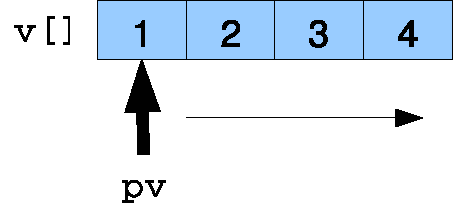
\includegraphics[width=5cm]{figures/pointer_array}
\caption{An illustration of a pointer being used to iterate over array elements, where the blue boxes signify the sequential sections of memory containing the values stored in the array.
\label{figure:pointer_array}}
\end{center}
\end{figure}

\subsection{Command Line}
A C program can either receive command line input at execution time or
by reading input from a file or other data source.  This example
demonstrates how command line arguments are passed into a C program
when the program is executed.  The design of the program is given as a
\flo in figure~\ref{figure:flowchart_ex4} and as \psc in
\psc~\ref{pseudo:ex4}. 

\begin{figure}[h]
\begin{center}
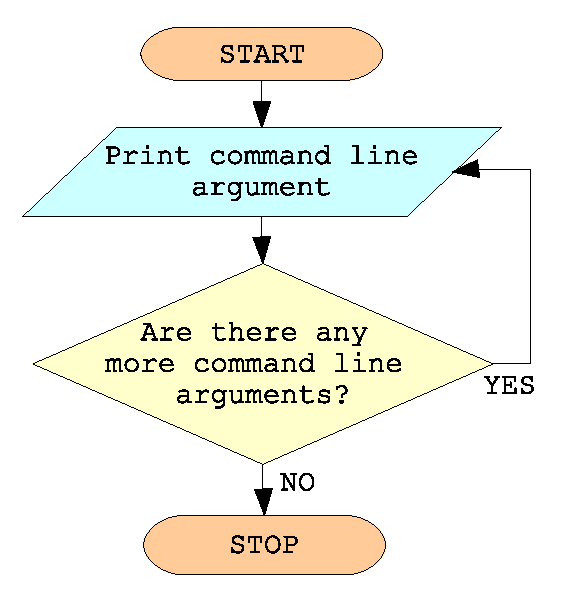
\includegraphics[height=5cm]{figures/ex4}
\caption{A flowchart describing example 4
\label{figure:flowchart_ex4}}
\end{center}
\end{figure}

\begin{pseudocode}[h]
\begin{verbatim}
main(command line arguments)
  Print the number of commmand line arguments
  Loop over the command line inputs
    Print each command line input
\end{verbatim}
\caption{Example 4 in pseudocode \label{pseudo:ex4}}
\end{pseudocode}

When programming C on a \linux\ platform the \main\ function is normally
implemented in one of two ways:
\begin{lstlisting}
int main(void)
\end{lstlisting}
and
\begin{lstlisting}
int main(int argc, char *argv[])
\end{lstlisting}
The second form allows command line input to be passed into the
program.  The operating system allocates the memory for
\texttt{*argv[]} and initialises it with the input command line
arguments.  The first element of the \texttt{argv} array contains the
name of the executable.  The second element exists only if there is a
argument following the name of the executable, etc.  The parameter
\texttt{argc} is initialised by the operating system with the number
of elements in the \texttt{argv} array.  While it may seem odd to
include the name of the executable in this list it can infact be
very useful.  For example, if a program has been written to do several
tasks a symbolic link can be used to control which task it performs.
The logic of this can be tested out using example 4 by typing
\begin{verbatim}
]$ ln -s command_line.exe another_cmd.exe
]$ ./another_cmd.exe
\end{verbatim}
A simple test on the value of \texttt{argv[0]} could then be used to
do something else.

\subsection{File access}
Most programs will need to save or read data from disk or another
input/output device.  Example 5 demonstrates how some simple data can
be written to and read from an ASCII file.  The design of the \main\ is given in figure~\ref{figure:flowchart_ex5} and the complete program is described in \psc~\ref{pseudo:ex5_main}~and~\ref{pseudo:ex5_fileio}.
\begin{figure}[h]
\begin{center}
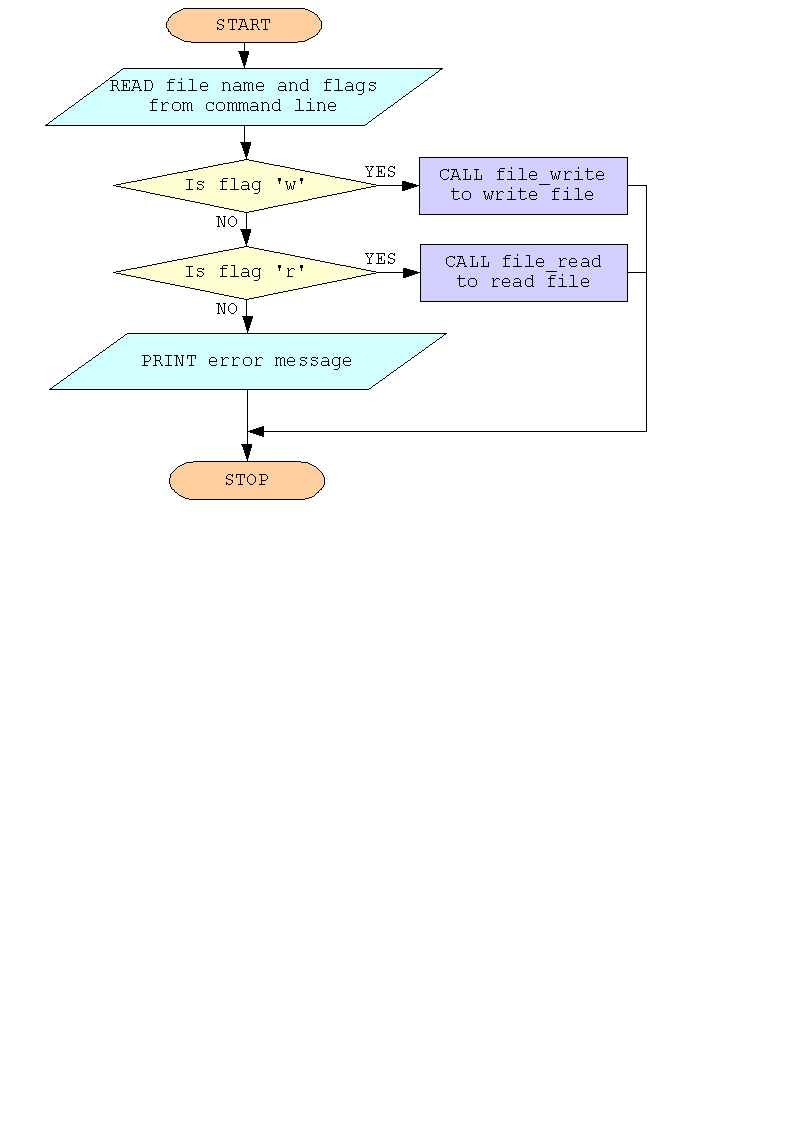
\includegraphics[height=7cm]{figures/ex5}
\caption{A flowchart describing the \main\ function of example 5
\label{figure:flowchart_ex5}}
\end{center}
\end{figure}

\begin{pseudocode}[h]
\begin{verbatim}
main(command line arguments)
  Check the command line arguments
    Make sure the file name is given
    Check for the input flag and if not given set the default to
    write.

  IF the input flag is write, write the specified file.
  ELSE IF the input flag is read, read the specified file.
  ELSE report an error
\end{verbatim}
\caption{The \main\ function of example 5 in pseudocode \label{pseudo:ex5_main}}
\end{pseudocode}

\begin{pseudocode}[h]
\begin{verbatim}
file_write(file name)
  Open an output file.
  IF the file was successfully opened
    LOOP from 1 to 20
      Print the value into the file.
      IF the value is a multiple of 5 then print a newline.
      ELSE print a space.
  ELSE
    Report an error.

file_read(file name)
  Open an input file.
  IF the file was successfully opened
    Get a character until the end of file or until the buffer is full.
    IF the character is not a space or a newline 
      Copy character into buffer.
    ELSE IF the buffer contains something
      Add a string terminating character.
      Scan the contents into an integer.
      Print the integer.
      IF the integer is a multiple of 5 print a new line.
      Reset the buffer.
  ELSE
    Report an error.
\end{verbatim}
\caption{The \texttt{file\_write()} and \texttt{file\_read()} functions of example 5 in pseudocode \label{pseudo:ex5_fileio}}
\end{pseudocode}

The program starts by checking the command line arguments.  Then
either \texttt{file\_write} or \texttt{file\_read} is called.  The
functions \texttt{file\_write} and \texttt{file\_read} are
pre-declared in the header file \texttt{file\_io.h} and implemented in
\texttt{file\_io.c}.  When this code is compiled the resultant machine
code \texttt{main.o} contains undefined references to these
functions.  Then at link time the machine code in \texttt{file\_io.o}
and \texttt{main.o} is linked together to produce the final
executable.  The practical process of building this executable is
discussed in section~\ref{section:make}.

\clearpage
\newpage

The \texttt{file\_io.h} header file of example 5 contains three pieces
of precompiler syntax which surround the function predeclarations.
\begin{lstlisting}
#ifndef FILE_IO_H
#define FILE_IO_H

void file_write(char *filename);
void file_read(char *filename);

#endif
\end{lstlisting} %$
The purpose of these statements is to prevent the functions from being
pre-declared twice.  While this does not happen within this example,
double declaration which can result in compiler errors is more of an
issue with more complicated programs.  It is therefore a good idea to
adopt the use of these precompiler statements at an early stage. 

The functions \texttt{file\_write} and \texttt{file\_read} are
implemented in \texttt{file\_io.c}.  The \texttt{file\_write} function
calls \texttt{fopen} to open a file for writing
\begin{lstlisting}
outputfile = fopen(filename,"w");
\end{lstlisting}
This command returns a {\em file pointer}, which is a pointer to a
\texttt{struct} \texttt{typedef} called \texttt{FILE}.  \texttt{FILE}
contains information about the file which needs to be passed between
the different file I/O function calls.  If the file cannot be opened
for writing then \texttt{null} is returned.  This is logically
equivalent to false and can therefore be used to check if the file was
opened correctly or not.
\begin{lstlisting}
if (outputfile) {
\end{lstlisting}
Once the file has been opened successfully data can be written in
ASCII format by calling the \texttt{fprintf} function.  This function
follows the same syntax as the \texttt{printf} function with the
exception of the {\em file pointer} as the first argument.  When all
the data have been written to the file \texttt{fclose} is called to
flush any remaining data in memory to the file and to close the file.
If \texttt{fclose} is not called, then when a program exits the file will
only be partially written to disk.

Once the output file is present on disk the function
\texttt{file\_read} is called to read the data back in and print them
to the standard out. \texttt{file\_read} starts by opening a file for
reading
\begin{lstlisting}
inputfile = fopen(filename,"r");
\end{lstlisting}
Then single characters are read from the file until the End Of File
(EOF) is reached or the character buffer is full.
\begin{lstlisting}
while((c=fgetc(inputfile)) != EOF  && j<9)
\end{lstlisting}
This is much more robust than just using \texttt{fscanf} to read data, which
can easily result in errors or crashes.  If the character is not a
space or a new line it is appended to the character buffer.  When a
space or a new line is found then if the buffer contains something it is
scanned into an \texttt{int} by calling
\begin{lstlisting}
sscanf(str, "%d", &i);
\end{lstlisting}
where \texttt{\&i} is the memory address of \texttt{i} and
\texttt{\%d} tells \texttt{sscanf} to treat the string as an integer.
After each \texttt{int} is read the data are printed back to the
standard output in the same form as they were saved to disk.  Finally
the file is closed.

\subsubsection{Make \label{section:make}}

As the number of files involved or dependencies increases simply
typing \texttt{gcc} would become an lengthy and complicated
task. Therefore from this example onwards \texttt{Make}\cite{make} is
used to aid with compilation and linking of examples.  The
\texttt{Makefile} in example 5 has three targets which can be called
from the command line:
\texttt{file\_io.exe}, \texttt{clean} and \texttt{veryclean}.  The
default target is the first one \texttt{file\_io.exe}.  The default
target it called by typing
\lstset{language=make}
\begin{verbatim}
]$ make
\end{verbatim} %$
The other targets are called by using the target name
\begin{verbatim}
]$ make veryclean
\end{verbatim} %$
Above the default target are the definition and initialisation of
three variables
\begin{lstlisting}
CC=gcc
TARGET=file_io
OBJECTS=main.o file_io.o
\end{lstlisting}
The last one of these is a list.  When the default target is called
the dependencies \texttt{\$(OBJECTS)} are checked.  If these files are
not found then \texttt{Make} looks through the file for a suitable
target to make these files with.  If there is a \texttt{.c} file with
the correct name it calls
\begin{lstlisting}
%.o: %.c
	@echo "**"
	@echo "** Compiling C Source" 
	@echo "**"
	$(CC) -c $(INCFLAGS) $<
\end{lstlisting} %$
This target compiles the \texttt{.c} file into a \texttt{.o} file.
Then when all of the \texttt{\$(OBJECTS)} are present on disk
\texttt{Make} executes the rest of the default target
\begin{lstlisting}
$(TARGET).exe: $(OBJECTS)
	@echo "**"
	@echo "** Linking Executable"
	@echo "**"
	$(CC) $(OBJECTS) -o $(TARGET).exe
\end{lstlisting} %$
which links the object files together to make the executable.

When any of the \texttt{.c} files referred to in the \texttt{Makefile}
are present but are newer than the \texttt{.o} file of the prefix
name, \texttt{Make} just rebuilds the files concerned and
completes the link step.  When any of the \texttt{\$(OBJECTS)} are
newer than \texttt{file\_io.exe}, \texttt{Make} just completes the
link step.  This can be tested out by using \texttt{touch}
\begin{verbatim}
]$ make
]$ touch main.c
]$ make
]$ touch file_io.o
]$ make
\end{verbatim} %$
More examples of \texttt{Make} syntax are given in later examples.

\lstset{language=C}

\clearpage
\newpage

\subsection{Problem}

While working in research it can often be the case that a piece of
equipment or software produces its output in the wrong form for use as
an input to another application.  The program
\texttt{problem/generator/generator.c} writes random numbers into a
\texttt{sample.txt} file.  Follow the instructions in
\texttt{generator/README} file to produce a \texttt{sample.txt}.  Then write a
program to convert \texttt{sample.txt} into a Comma Separated Values file (CSV)\cite{csv} suitable for use as input to a spreadsheet.  Run your program and read the resultant output into a spreadsheet and plot the Value column as a histogram.

Start by drawing a simple \flo\ outline of the program.  Then write the program in \psc.  Finally write your program in C using code from each of this section's examples as necessary.  Remember to add comments.

\clearpage
\newpage

%%%%%%%%%%%%%%%%%%%%%%%%%%%%%%%%%%%%%%%%%%%%%%%%%%%%%%%%%%%%%%%%%%%%%%%%%%%%

\section{Data structures}
In this section more complex data structures \texttt{struct} and \texttt{union} will
be discussed.  An example of how to interface to FORTRAN77 code will
be given and the section finishes with a complicated example including
much of the syntax introduced so far.

\subsection{Pointers and structs}

The purpose of example 6 program is to demonstrate \texttt{struct} syntax
and to show how arrays and \texttt{struct}s can be passed into a
function.  The program is described by \psc~\ref{pseudo:ex6}.

\begin{pseudocode}[h]
\begin{verbatim}
main()
  Instantiate two ints, an array of two ints and two structs.
  Assign 1 to all data members
  Print the values contained in the ints, the array and the structs
  Call fun() to modify some of the values
  Print the values contained in the ints, the array and the structs

fun(int np, int *p, int *arr, struct st dat, struct st *dat_ptr)
  Change the value of the local variable np
  Change the value in the memory p points to.
  Change the values of the two elements of arr
  Change the data members of the local struct dat
  Change the data members of the struct dat_ptr points to.
\end{verbatim}
\caption{Example 6 in pseudocode \label{pseudo:ex6}}
\end{pseudocode}

At the top of the file \texttt{pointers2.c} a struct is defined
\begin{lstlisting}
struct st {
  int i;
  int array[2];
};
\end{lstlisting}
where \texttt{st} is the name of the \texttt{struct}.  The data
members of the struct are enclosed in the \texttt{\{\}} brackets.  This
definition can be given in a header file instead of in a source file.
The definition defines the \texttt{struct} but does not create an
instance of it.  Then in the \main two \texttt{st} \texttt{struct}s
are instantiated
\begin{lstlisting}
struct st dat, dat_p;
\end{lstlisting}
and their data members are initialised.
\begin{lstlisting}
dat.i=1;
dat.array[0]=1;
dat.array[1]=1;
dat_p.i=1;
dat_p.array[0]=1;
dat_p.array[1]=1;
\end{lstlisting}
The syntax is {\em $<$instantiation$>$.$<$data~member$>$}.  Each instantiation
of a \texttt{struct} is stored in a separate block of memory.  Unlike an array
the data members can have different lengths.  The total memory used by a
\texttt{struct} instantiation is determined by the sum of the memory
used for the data members.  The order of the \texttt{struct} members in
the \texttt{struct} definition determines the order of their allocation in
memory.  The member types can include other \texttt{struct}s,
\texttt{union}s, arrays and basic variables etc..

After the \texttt{struct}s, basic variables and the array have all been
initialised the function \texttt{fun()} is called.  This function is
called with the value of \texttt{np}, the address of \texttt{p}, the
array \texttt{arr}, the value of \texttt{dat} and the address of
\texttt{dat\_p}.  Notice that the name of the array \texttt{arr} is actually
equivalent to passing an address of the first element
\texttt{\&arr[0]}.  Therefore the function declaration and
implementation of \texttt{fun} includes this as \texttt{int~*}.
Inside the function \texttt{fun} each of the variables is given a
different value.  The syntax of accessing data members of a
\texttt{struct} pointer is 
{\em $<$pointer~name$>-><$data~member$>$} 
\begin{lstlisting}
dat_ptr->i=5;
\end{lstlisting}
or 
{\em (*$<$pointer~name$>$).$<$data~member$>$}
\begin{lstlisting}
(*dat_ptr).i=5;
\end{lstlisting}
When the function \texttt{fun} is called the argument
\texttt{struct~st~dat} caused a new instantiation of the
\texttt{struct~st} to be made.
\begin{lstlisting}
void fun(int np, int *p, int *arr, struct st dat, struct st *dat_ptr) {
\end{lstlisting}
The memory assigned to this instantiation is local to the function
\texttt{fun} and will go out of scope when the program leaves this
function.  When the function is called the data members of
\texttt{dat} are initialised with the values of the data members of
\texttt{dat} from the \main.  The behaviour is therefore similar to
the variable \texttt{np}.

Unlike \texttt{dat}, the address of \texttt{dat\_p} is passed into
the function fun.  The pointer\\
\texttt{struct~st~*dat\_ptr} is therefore initialised with this
address.  When the data members of the 
object that \texttt{*dat\_ptr} points to are modified
\begin{lstlisting}
dat_ptr->i=5; dat_ptr->array[0]=6; dat_ptr->array[1]=7;
\end{lstlisting}
then the change is still present when the execution returns to the
\main.

\subsection{Binary I/O and unions}
In example 7 the data concerning several fundamental particles are
written in binary form into an output file.  Then the program reads
these data back and prints out the 7$^\mathrm{th}$ particle data record.  The design of the program is given in \psc~\ref{pseudo:ex7}.

\begin{pseudocode}[h]
\begin{verbatim}
main()
  Print the size of one union entry.
  Print the size of each union member.
  Write 10 records of fundamental particles to a binary file.
  Read the 7th record back from the binary file.
  Print the values of the 7th record.

status write_records()
  Create an array of 12 records.
  Initialise the array of records with fundamental particle data.
  Open a file for writing.
  Write each record element out in binary form.
  Close the file.

status find_record()
  Open an input file.
  Fast forward to the 7th record.
  Read the 7th record.
  Close the file.
\end{verbatim}
\caption{Example 7 in pseudocode \label{pseudo:ex7}}
\end{pseudocode}

At the beginning of the \main\ a \texttt{record} \texttt{dat} is
instantiated.
\begin{lstlisting}
record dat;
\end{lstlisting}
\texttt{record} is a \texttt{typedef} declared in the header file
\texttt{data\_record.h}.
\begin{lstlisting}
typedef entry record[4];
\end{lstlisting}
This statement means that a \texttt{record} is a \texttt{typedef} of
an array of \texttt{entry}s of length 4.  Therefore
\begin{lstlisting}
record dat;
\end{lstlisting}
is equivalent to
\begin{lstlisting}
entry dat[4];
\end{lstlisting}
The type \texttt{entry} is itself a \texttt{typedef} of a union
\begin{lstlisting}
typedef union {
  int id;
  double mass;
  char name[16];
  int charge;
} entry;
\end{lstlisting}
In the previous example \texttt{struct}s were declared with the syntax:
\begin{lstlisting}
struct st {

};
\end{lstlisting}
This syntax is allowed with \texttt{union}s and the \texttt{union}
syntax used in this example is allowed with \texttt{struct}s.
\begin{lstlisting}
typedef struct {

} st;
\end{lstlisting}
The advantage of the \texttt{typedef} form used in this example is
that the \texttt{union} prefix does not have to be carried around the
code.  It is therefore much more common that the \texttt{typedef} form
of a \texttt{struct} or \texttt{union} definition is used.

A \texttt{union} contains a set of members which are listed within the
\texttt{\{\}} brackets.  The members of a \texttt{union} share the same memory allocation.  The size of the \texttt{union} is therefore set by the largest member.  This can easily be demonstrated by running example 7.  The syntax for accessing the members of a \texttt{union} is the same as the syntax used for accessing the members of a \texttt{struct}.

In this example an array of the \texttt{entry} \texttt{union} is
created with 4 elements, this is a \texttt{record}.  The
\texttt{record} stores a particle's \texttt{id}, \texttt{mass},
\texttt{name}, and \texttt{charge}.  To make the code more readable a
set of \texttt{\#define} statements are used instead of the indices.
\begin{lstlisting}
#define RECORD_ID 0
#define RECORD_MASS 1
#define RECORD_NAME 2
#define RECORD_CHARGE 3
\end{lstlisting}
When the code compiles the precompiler replaces each
definition with its value.  Then the compiler turns the result into
machine code.  It is a common convention that \texttt{\#define}
statements use all upper case letters to avoid confusion with real
variables.  What follows the \texttt{\#define~NAME} does not have to
be a simple number, the precompiler just does a find and replace.

The first use of the precompiler definitions is in
\texttt{write\_records}.  In this function an array of \texttt{record}s is
instantiated
\begin{lstlisting}
record particle_data[12];
\end{lstlisting}
and each \texttt{entry} is filled by simple assignment.
\begin{lstlisting}
particle_data[0][RECORD_ID].id = 22;
particle_data[0][RECORD_MASS].mass = 0.E+00;
strcpy(particle_data[0][RECORD_NAME].name,"gamma");
particle_data[0][RECORD_CHARGE].charge = 0;
\end{lstlisting}
This demonstrates that the array index contained in the
\texttt{typedef}~\texttt{record} statement comes after the array index
defined by defining the \texttt{particle\_data} array.

Following the initialisation of the \texttt{particle\_data} array the
data are written to a binary file.  The binary file is opened in the
same way as the ASCII file in example 5.
\begin{lstlisting}
file_ptr = fopen(particle_file,"w");
\end{lstlisting}
This time however the error messages are handled by printing them to
the standard error.  To print to the standard error the
\texttt{fprintf} function is used with the standard error {\em file
pointer} \texttt{stderr}.
\begin{lstlisting}
fprintf(stderr," Error: unable to open \'%s\' for writing.\n", particle_file);
\end{lstlisting}
The standard error is printed to the console or shell window in the
same manner as the standard output but is contained in a different
stream.  When running a program on \linux\ the standard output an be redirected to a file.
\begin{verbatim}
]$ ./prog.exe > output
\end{verbatim} %$
This does not redirect the standard error though, which can be left
for the user to read.\footnote{It is possible to redirect both
standard error and standard output to one file.}

Once the file has been opened the \texttt{particle\_data} records are written to it in binary form.
\begin{lstlisting}
fwrite(&particle_data[i][j], 16, 1, file_ptr);
\end{lstlisting}
The arguments of \texttt{fwrite} are the address of one \texttt{union}
instantiation, the size of the \texttt{union}, the number of
\texttt{union} instantiations to be written and the {\em file pointer} to which the data should be written.  Since the size of the \texttt{union} is set by the largest member each data element is the same size.  This means that the code to write out these data is very simple and only requires two loops over the \texttt{fwrite} statement.  

After the data have been written to disk \texttt{find\_record} is
called to find and read the 7th record.  \texttt{find\_record} opens
the binary file in the same way as the ASCII file was opened in
example 5.
\begin{lstlisting}
file_ptr = fopen(particle_file,"r"); 
\end{lstlisting}
Then after checking the file was opened successfully it fast forwards to the correct position in the file
\begin{lstlisting}
if(fseek(file_ptr, (long)(sizeof(*dat)*offset), 0) != 0)
\end{lstlisting}
where \texttt{fseek} returns a non-zero value if the seek fails.  This then leaves the file-position indicator set to point at the value given by the offset.  The record is then read by calling \texttt{fread}.
\begin{lstlisting}
fread(dat, sizeof(*dat), 1, file_ptr);
\end{lstlisting}
Finally in the \main\ these data are printed to the standard out
\begin{lstlisting}
printf("\t Id \t Mass    \t Name          \t Charge \n");
printf("\t %d \t %3.3e \t %-12s \t %d \n", 
       dat[RECORD_ID].id,
       dat[RECORD_MASS].mass,
       dat[RECORD_NAME].name,
       dat[RECORD_CHARGE].charge);
\end{lstlisting}

Throughout example 7 possible errors are caught and result in a
non-zero value being returned to the operating system.  When writing
a program it is important to make sure the implementation is able to
prevent crashes by handling error conditions properly.  This means
that the program should exit in a controlled manner and provide the
user with a description of the error, rather than a cryptic message or nasty crash.

\subsection{Linking with FORTRAN77}

Although many modern programs have been written in C it is sometimes
very useful to be able to link C code to another programming language.  When the code to be linked to is compiled into machine code this can be achieved by knowing how the two compilers concerned work.  For example, FORTRAN77 a programming language often used for physics and engineering applications, can be compiled by \texttt{g77} into object files.  These object files can be browsed with \texttt{nm}.  
\begin{verbatim}
]$ g77 -c fortran.for
]$ nm -g fortran.o 
00000251 T call_back__
00000000 T commons_
         U do_lio
         U e_wsle
00000062 C forcom_
         U mult_a__
         U s_wsle
\end{verbatim}
C code is also compiled into object files, which can also be browsed
with \texttt{nm}.
\begin{verbatim}
]$ gcc -c main.c 
]$ nm -g main.o
         U call_back__
         U commons_
00000065 T fill_common
         U forcom_
00000000 T main
000000ed T mult_a__
         U sprintf
\end{verbatim}
All that is needed to join FORTRAN77 with C is for the undefined
references in FORTRAN77 or C to be present in the object files
generated from the other language.  In this example
\texttt{call\_back\_\_}, \texttt{commons\_}, \texttt{forcom\_} and
\texttt{mult\_a\_\_} are linked between the two languages.  The other
undefined symbols can be found in the system libraries.  When
\texttt{g77} compiles the FORTRAN code it uses a lower case version of
the name and appends one underscore to  the end of the name or two
underscores if the name already contains an underscore.\footnote{This
behaviour can be controlled by using compiler options.}

Example 8 demonstrates all of the features of linking C and FORTRAN77
together.  The design of the program is given in \psc~\ref{pseudo:ex8}.

\begin{pseudocode}[h]
\begin{verbatim}
main()
  Fill the FORTRAN common block with numbers and a string.
  Print the contents of the FORTRAN common block with FORTRAN code.
  Multiply a number and print a string by calling the FORTRAN code.

fill_common()
  Fill the int and float arrays of the common plot with 
    sequential numbers.
  Fill the FORTRAN string with a C string.

mult_a__()
  Multiply the input value by 10 and return it.

SUBROUTINE COMMONS
  Print the contents of the common block.

FUNCTION CALL_BACK
  Print the input string.
  Call the C function to multiply the input value by 10.
  Print the resulting value and return it.
\end{verbatim}
\caption{Example 8 in pseudocode \label{pseudo:ex8}}
\end{pseudocode}

There are some important differences to point out between the two
languages.  Firstly C strings are character arrays terminated by the
'\texttt{$\backslash$0}' character.  This means that the maximum
length of a string is equal to the number of elements of the character
array minus one.  In FORTRAN character arrays are also used to store
strings but unlike C '\texttt{$\backslash$0}' is not used.  The
maximum length of a string in FORTRAN is therefore set by the number
of elements in the character array.  FORTRAN keeps track of the length
of a string by implicitly passing its length with the string.  When
FORTRAN is compiled with g77 these implicit variables become explicit
in the machine code output.  Therefore when calling a FORTRAN function
from C, the lengths of each of the strings must follow each of the
character arrays:
\begin{lstlisting}
float call_back__(float *,char *, int);
\end{lstlisting}
where the int is the implicit string length variable.

The allocation of memory to FORTRAN arrays is different to that of C.
For example when a two dimensional array is declared in FORTRAN
\lstset{language=Fortran}
\begin{lstlisting}
INTEGER INTARRAY(3,2)
REAL REALARRAY(2,3)
\end{lstlisting}
\lstset{language=C}
in C the array indices of the equivalent memory mapping are:
\begin{lstlisting}
int intarray[2][3];
float realarray[3][2];
\end{lstlisting}
The first index of a FORTRAN array is by default 1, but C always uses
0 as the first index of an array.  These differences are particularly
important when dealing with \texttt{common} blocks.  In the FORTRAN
include file \texttt{FORTRAN.INC} a common block is declared.
\lstset{language=Fortran}
\begin{lstlisting}
INTEGER INTARRAY(3,2)
REAL REALARRAY(2,3)
CHARACTER*50 SOMESTRING
COMMON/FORCOM/INTARRAY,REALARRAY,SOMESTRING
\end{lstlisting}
\lstset{language=C}
This defines the common block and creates one global instance of the
common block in memory.  In a similar fashion to a \texttt{struct}, the
order of the member variables denotes there order in memory, and the total
size of the common block is just the sum of the sizes of the members.
Once a common block has been declared FORTRAN or C code can access its
data members.  The FORTRAN common block can be included in several
different FORTRAN files, but only one instance of it will be created
in memory.  This global memory can be accessed from C by creating a
global un-resolved \texttt{struct} of the correct name.
\begin{lstlisting}
typedef struct {
  int intarray[2][3];
  float realarray[3][2];
  char somestring[50];
} forcom;

extern forcom forcom_;
\end{lstlisting}
The \texttt{extern} command means that the compiler will look through
the object files for the memory definition of \texttt{forcom\_} and
link to it, rather than allocate another block of memory.  Without the
\texttt{extern} prefix the memory allocated in the C program would be
different to that of the FORTRAN common block.  The order, types and
sizes of the C \texttt{struct} must match the order, types and sizes of the
FORTRAN common block.

In addition to the memory mapping and variable type name differences,
FORTRAN uses pointers implicitly in function calls.  A function
of the form
\lstset{language=Fortran}
\begin{lstlisting}
FUNCTION CALL_BACK(A,NAME)
IMPLICIT NONE
REAL A, C, CALL_BACK, MULT_A
CHARACTER*(*) NAME
\end{lstlisting}
\lstset{language=C}
is therefore equivalent to
\begin{lstlisting}
float call_back__(float *,char *, int);
\end{lstlisting}
The last variable in the C version of this function is the length of
the string, which is implicitly present in the FORTRAN code.  

\subsection{Sine wave generator}
As programs become larger the initial design becomes more important.
Therefore to encourage thought about program structure the example
programs given in this course will become more and
more complicated.  In  example 9 there are 9 C files containing a
total of 300 lines.  When writing a program of this size it needs to
be clear what the design requirements and components are.

\subsubsection*{Design}

\paragraph{Requirements}
A program to either generate sine wave spectra and save them to a
binary file or read the spectra from a binary file.  The last
spectrum either written to or read from the file should be plotted with
gnuplot~\cite{gnuplot}.

\paragraph{Components}
\begin{itemize}
\item \texttt{main} implement in \texttt{main.c}\\
Handles the users command line arguments and selects either write or
read with the selected number of events if this is given.\\
%
\item \texttt{gen\_data} implement in \texttt{gen\_data.c}\\
Generates the sine wave from a flat random number generator\\
%
\item \texttt{gen\_value} implement in \texttt{gen\_data.c}\\
A function to generate a random floating point number between two 
limits using a flat random number generator.\\
%
\item \texttt{write\_data} implement in \texttt{file\_io.c}\\
A function to write a data sample to a binary file \\
%
\item \texttt{read\_data} implement in \texttt{file\_io.c}\\
A function to read a data sample from a binary file\\
%
\item \texttt{sample} define in \texttt{gen\_data.h} \\
A struct to contain sine wave samples.\\
%
\item \texttt{plot\_data} implement in \texttt{plot\_data.c} \\
A function to plot a data sample with gnuplot \\
%
\item \texttt{gnuplot} implement in \texttt{gnuplot.c} \\
A function to provide an interface with gnuplot by using a system
call. \\
\end{itemize}

\subsubsection*{Discussion of the implementation}
The implementation of example 9 is described in
\psc~\ref{pseudo:ex9_main}, \ref{pseudo:ex9_gen_data},
\ref{pseudo:ex9_file_io} and \ref{pseudo:ex9_plot_data}.

\begin{pseudocode}[h]
\begin{verbatim}
main(commmand line inputs)
  Check the command line inputs
    IF the file name and flag are not given report an error
    IF the flag is -w check for the number of events
      IF the number of events has not been given set it to 10 events.
      ELSE read the number of events.
      Open an output file.
      Write the number of events into the file as a header.
      Generate the required number of events needed.
         Write each one to the output file.
    
      Plot the last event with gnuplot.
      close the output file.

    ELSE IF the flag is -r open an input file.
      Read the number of events, recorded at the start of the file.
      IF the number of events has not been given use the number at the
        top of the file.
      ELSE check if the argument is a number and if it is set the
        number of events to read to be the number given.
      IF the number of events selected is greater than the number of
        events in the file
        Set the number of events selected to be the number of events 
          in the file. 

      Read the events from the file.
      Plot the last event.
      Close the input file.
   ELSE return an error reporting the flag is invalid.
\end{verbatim}
\caption{Example 9 in pseudocode \label{pseudo:ex9_main}}
\end{pseudocode}

\begin{pseudocode}[h]
\begin{verbatim}
gen_value(limits)
  Generate a random float between two limits using a flat random
    distribution. 
  Return this value

gen_data(data sample pointer)
  Set the limits for the random parameters: number of points, a, b, and c.
  Generate values for: the number of points, a, b, and c.
  Use the number of points to determin the step size, where the range
    of x is 0 to 2PI.
  Use the step size, and the values for a, b, and c to generate the
    sine wave event.
\end{verbatim}
\caption{Example 9 in pseudocode \label{pseudo:ex9_gen_data}}
\end{pseudocode}

\begin{pseudocode}[h]
\begin{verbatim}
write_data(file pointer, data record)
  Write the number of points
  Loop over all points
    Write the x value
    Write the y value

read_data(file pointer, data record)
  Read the number of points
  Loop over all points
    Read the x value
    Read the y value
\end{verbatim}
\caption{Example 9 in pseudocode \label{pseudo:ex9_file_io}}
\end{pseudocode}

\begin{pseudocode}[h]
\begin{verbatim}
plot_data(data record)
  Open a temporary output file.
  Loop over all points
    Write "x y" as text to the file.
  Create the gnuplot command.
  Plot the data with gnuplot.
  Remove the temporary output text file.
\end{verbatim}
\caption{Example 9 in pseudocode \label{pseudo:ex9_plot_data}}
\end{pseudocode}

This program uses several concepts that were introduced with
previous examples.  The discussion of this example therefore only
covers additional points.

The program starts by checking if a binary file is to be written or
read.  It then checks the number of events which should be either
written or read.  Following this the program writes or reads sine wave
data to or from the binary file and plots the last sine wave sample with
gnuplot.  In example 9 the each sine wave sample is stored in an
instantiation of a \texttt{struct}~\texttt{typedef}~\texttt{sample}.
\begin{lstlisting}
typedef struct {
  float x[MAX_PTS]; /* The x value */
  float y[MAX_PTS]; /* The y value */
  int pts; /* Number of points in the sample */
} sample;
\end{lstlisting}
In the \main an instance of \texttt{sample} is declared.
\begin{lstlisting}
sample dat;
\end{lstlisting}
Then \texttt{dat} is either filled with generated data
\begin{lstlisting}
gen_data(&dat);
\end{lstlisting}
or with data read from a file.
\begin{lstlisting}
read_data(file_ptr, &dat);
\end{lstlisting}
While sizes of the data member arrays \texttt{x} and \texttt{y} are
fixed the number of elements used varies.  Therefore the data member
\texttt{pts} is use to keep track of the number of useful elements in
memory.  When these data are written to file the record length of each
sine wave sample varies in accordance with the value of \texttt{pts}.
The value of \texttt{pts} is therefore written to the file for each
sine wave sample.  An illustration of the resultant file structure is given in
figure~\ref{figure:ex9_file_structure}.
%
\begin{figure}[h]
\begin{center}
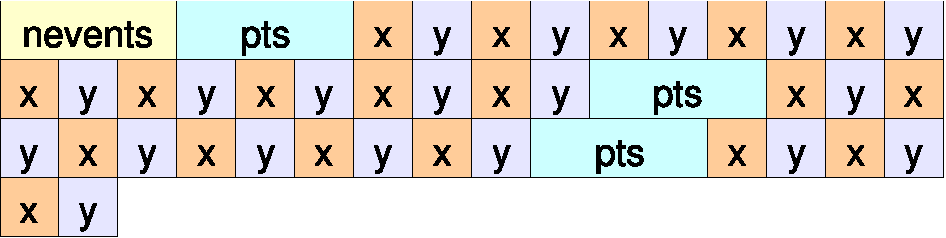
\includegraphics[width=12cm]{figures/ex9_file_structure}
\caption{An illustration of the binary file structure used in example 9
\label{figure:ex9_file_structure}}
\end{center}
\end{figure}

The last sine wave sample that is either read from file or generated
is plotted with gnuplot.  The \main calls \texttt{plot\_data}, passing
it a pointer to the last sample.   \texttt{plot\_data} then writes a
temporary file for gnuplot to read.  This file has to be of the form:
``\texttt{$<$number$>$ $<$number$>$}''.  Then after plot\_data has
written the file the gnuplot command is assembled.
\begin{lstlisting}
sprintf(gnuplot_command, "plot \'%s\'\n", filename);
\end{lstlisting}
(\texttt{sprintf} follows the same syntax as \texttt{printf} but starts
with a pointer to a string buffer.)  The command assembled corresponds
to what would be typed at the interactive gnuplot command line to plot
these data.  This command is passed to the \texttt{gnuplot} function
to plot the data.  The \texttt{gnuplot} function inserts another
string in front of the gnuplot command
\begin{lstlisting}
sprintf(syscommand, "echo \"%s\" | gnuplot -persist", gnucommand);
\end{lstlisting}
and uses a system call to execute the command in a \linux\ shell.
\begin{lstlisting}
system(syscommand);
\end{lstlisting}
The affect of the ``\texttt{-persist}'' is that gnuplot continues to
run after the C program has exited. 

\clearpage
\newpage

\subsection{Problem}
Programs are often written to interface with hardware, for slow control or 
data acquisition.  Since the \linux\ lab does not contain any external 
hardware this problem concerns monitoring the computer itself.

A program is provided which requests more and more memory by calling
\texttt{malloc}.  After some period of time the program then frees the
dynamically allocated memory by calling \texttt{free}.  Write a
program to monitor the total memory used every second for a given
number of minutes.  The program should finish by plotting the total
memory usage as a function of time.  Once the pseudocode and
implementation has been finished run the monitoring program at the
same time as the memory loading program:
\begin{verbatim}
]$ ./system_monitor.exe 2 &
]$ ../problem/resource_hog/resource_hog.exe
\end{verbatim}
where 2 is the number of minutes the monitoring program should run.

\subsubsection*{Hints}
The memory allocation status can be obtained by calling \texttt{sysinfo}
\begin{lstlisting}
int sysinfo (struct sysinfo *info)
\end{lstlisting}
This function can be called by including
\begin{lstlisting}
#include <sys/sysinfo.h>
\end{lstlisting}
This include file also includes a definition of the \texttt{sysinfo} struct:
\begin{lstlisting}
struct sysinfo {
  long uptime;             /* Seconds since boot */
  unsigned long loads[3];  /* 1, 5, and 15 minute load averages */
  unsigned long totalram;  /* Total usable main memory size */
  unsigned long freeram;   /* Available memory size */
  unsigned long sharedram; /* Amount of shared memory */
  unsigned long bufferram; /* Memory used by buffers */
  unsigned long totalswap; /* Total swap space size */
  unsigned long freeswap;  /* swap space still available */
  unsigned short procs;    /* Number of current processes */
  unsigned long totalhigh; /* Total high memory size */
  unsigned long freehigh;  /* Available high memory size */
  unsigned int mem_unit;   /* Memory unit size in bytes */
  char _f[20-2*sizeof(long)-sizeof(int)]; /* Padding for libc5 */
};
\end{lstlisting}
%
Use the \texttt{sleep} command used in
\texttt{problem/resource\_hog/main.c} to sleep for 1 second between
measurements.  This will prevent the monitoring program from using
up a lot of CPU, which would affect the results.  More information can
be found in the manual page by typing
\begin{verbatim}
]$ man -s 3 sleep
\end{verbatim} %$
%
Use the \texttt{time} command used in
\texttt{problem/resource\_hog/main.c}.  More information can be found
in the in the manual page by typing
\begin{verbatim}
]$ man time.h
\end{verbatim} %$

\clearpage
\newpage

%%%%%%%%%%%%%%%%%%%%%%%%%%%%%%%%%%%%%%%%%%%%%%%%%%%%%%%%%%%%%%%%%%%%%%%%%%%%
\section{Simple analyses}
During previous sections much of the C programming language has been
introduced.  This section is therefore dedicated to solving more
complicated problems.

\subsection{Histogramming data}

When processing large volumes of data it is often very useful to
accumulate data values in histograms.  Histograms provide an important
tool for observing fluctuations in a data sample.  For example, a
histogram could be used to find a mass peak above a flat background.

Example 10 is a program to histogram the output of two random number
generators.  Its design and implementation are discussed in the
following sub-sections.

\subsubsection*{Design}

\paragraph{Requirements}
A program to histogram random numbers generated according to uniform
and Gaussian distributions.  The program should provide these random
numbers by using the integer random number generator \texttt{rand}
from \texttt{stdlib.h}.  The histrogramming code should provide visual
output using \texttt{gnuplot}.

\paragraph{Components}
\begin{itemize}
\item \texttt{main} implement in \texttt{main.c}: 
create two histograms and fill them with 10000 uniform and Gaussian
random numbers respectively.  Display the results with
\texttt{gnuplot}.
%
\item Provide histogram functionality.
\begin{itemize}
\item \texttt{hist\_create} implement in \texttt{histogram.c}:
a function to create a histogram 
%
\item \texttt{hist\_book} implement in \texttt{histogram.c}:
a function to add a value to an existing histogram 
%
\item \texttt{hist\_plot} implement in \texttt{histogram.c}:
a function to plot a histogram's contents using gnuplot. 
%
\item \texttt{hist\_entry} define in \texttt{histogram.c}:
a \texttt{struct} to contain the information of each histogram.
%
\item \texttt{gnuplot} implement in \texttt{gnuplot.c}: 
A function to provide an interface with gnuplot by using a system
call.
%
\end{itemize}
%
\item Provide random number  functionality.
\begin{itemize}
\item \texttt{set\_seed} implement in \texttt{random\_dist.c}:
a function to set the seed of the random number generator.
%
\item \texttt{random\_dist\_flat} implement in
\texttt{random\_dist.c}:
a function to return a floating point random number between 0. and 1.
%
\item \texttt{random\_dist\_gaus} implement in
\texttt{random\_dist.c}:
a function to return a floating point random number following a
Gaussian distribution with a given sigma.
\end{itemize}
\end{itemize}

\subsubsection*{Discussion of the implementation}
The implementation of example 9 is described in
\psc~\ref{pseudo:ex10_main}, \ref{pseudo:ex10_histogram}, and
\ref{pseudo:ex10_random_dist}.

\begin{pseudocode}[h]
\begin{verbatim}
main()
  Create two histograms.
  Loop for 10000
    Generate a random number following a Gaussian distribution.
    Histogram the Gaussian random number.
    Generate a random number following a uniform distribution.
    Histogram the uniform random number.
  Plot both histograms using gnuplot
\end{verbatim}
\caption{Example 10 in pseudocode \label{pseudo:ex10_main}}
\end{pseudocode}

\begin{pseudocode}[h]
\begin{verbatim}
hist_create(histogram name, number of bins, lower limit, upper limit)
  Fill static memory with histogram information.
  Calculate bin size and store it in static memory.
  Initialise all bins to be 0.
  RETURN this histogram's index

hist_book(histogram index, value, weight)
  IF the value is less than the lower limit increment the underflow
    bin by the weight.
  ELSE IF the value is greater or equal to the upper limit increment
    the overflow bin by the weight.
  ELSE find which bin the value is inside and increment its value by
    the weight.

hist_plot(histogram index)
  Create a temporary file for gnuplot
  Open the temporary file
  Save the data as "<value> <value>" to the file.
  Assemble a gnuplot command to plot the histogram.
  Call gnuplot.
  Remove the temporary file.
\end{verbatim}
\caption{Example 10 in pseudocode \label{pseudo:ex10_histogram}}
\end{pseudocode}

\begin{pseudocode}[h]
\begin{verbatim}
random_dist_flat()
  Generate an integer random number
  Use the limit of the integer to calculate a floating point number
    between 0 and 1.
  RETURN the floating point number.

random_dist_gaus(double sigma)
  IF a spare random number is not present
    Generate two random numbers within the unit circle.
    Use a Box-Muller transformation to get two Gaussian random
      numbers. 
    Save one of the random numbers in static memory and RETURN the
      other.
  ELSE
    RETURN the spare random number. 
\end{verbatim}
\caption{Example 10 in pseudocode \label{pseudo:ex10_random_dist}}
\end{pseudocode}

The program starts by creating two histograms.
\begin{lstlisting}
hist_create("Gaus",20,-3.0,3.0);
hist_create("Flat",20,0.0,1.0);
\end{lstlisting}
The \texttt{hist\_create} function assigns the histogram information
to members of an element of the \texttt{h\_dat} array.  The variable
\texttt{num\_hist} is used to keep track of which elements of
\texttt{h\_dat} array have been filled.  Both \texttt{h\_dat} and
\texttt{num\_hist} are globally available within
\texttt{histogram.c}.  
\begin{lstlisting}
static int num_hist = 0;
static hist_entry h_dat[MAX_HIST];
\end{lstlisting}
The \texttt{static} prefix means that no function outside
\texttt{histogram.c} is able to access these variables.  Without the 
\texttt{static} prefix the variables could be accessed by a function
implemented outside \texttt{histogram.c} provided an \texttt{external}
instantiation was used.  An example of an \texttt{external}
instantiation is given in example 8.

The advantage of instantiating \texttt{h\_dat} and
\texttt{num\_hist} globally in \texttt{histogram.c} is that they do
not go out of scope.  Therefore every time one of the histogram
functions is called \texttt{h\_dat} and
\texttt{num\_hist} are still in memory.

The variable \texttt{h\_dat} is an array of \texttt{typedef}
\texttt{struct} \texttt{hist\_entry}, which is defined in
\texttt{histogram.c} rather than in a header file.  The reason
for this is that \texttt{hist\_entry} is intended just for storing
histogram information.  When writing a large program it is highly
advisable to break it down into building blocks.  In this program the
histogram functions and the associated data are one building block.

Once the histograms have been created a Gaussian random number is
generated by calling \texttt{random\_dist\_gaus()}.  When this
function is called it either generates two random numbers and returns
one, or uses the spare one stored from the last time it was called.  To
store the spare random number \texttt{random\_dist\_gaus()} uses two
static variables:
\begin{lstlisting}
static int random_dist_gaus_status = 0;
\end{lstlisting}
and
\begin{lstlisting}
static double spare_num;
\end{lstlisting}
The variable \texttt{random\_dist\_gaus\_status} is defined outside
the function \texttt{random\_dist\_gaus()} as \texttt{static}.  It is
therefore private to the functions within \texttt{random\_dist.c}.
The variable \texttt{spare\_num} is defined as \texttt{static} within
the function \texttt{random\_dist\_gaus()}.  Unlike normal local
variables the variable \texttt{spare\_num} is defined once in memory
and does not go out of scope when the program leaves the
\texttt{random\_dist\_gaus()} function.  The value stored in
\texttt{spare\_num} at the end of \texttt{random\_dist\_gaus()} is
therefore available when the function is next called.

There are some program operations that can cause a serious error.
For example, if an array index is outside of the arrays memory
allocation or if a function is passed a variable outside of the limits
allowed.  Wherever program structures or function calls are used
that might cause such an error they should be protected.  In example
10 there is a simple catch to prevent an array index from going out of
bounds.
\begin{lstlisting}
if(i<0) {
  fprintf(stderr,"CRITICAL ERROR: something has gone very wrong!\n");
  exit(1);
}
h_dat[h_index].bins[i] += weight;
\end{lstlisting}
The program should not ever get inside this \texttt{if} statement.  If
it does there is a serious bug in the code.  The \texttt{exit(1)}
function call causes the program to terminate and return 1 to the
operating system.  This is a rather extreme case and other error
prevention code may not need to cause the program to exit.  For
example, if a section of code is written to calculate the hypotenuse
of a right angled triangle, then the code should catch the case where
the sides have no length.
\begin{lstlisting}
double a, b=0., c=0.;
double a_sqd; /* a squared */
a_sqd = pow(b,2.0)+pow(c,2.0); /* b^2 + c^2 */
if(a_sqd<=0) { /* Prevent a possible sqrt error */
  a = 0;
}
else {
  a = sqrt(a_sqd);
}
\end{lstlisting}

After the histograms have been filled \texttt{hist\_plot} is called to
plot this histogram using gnuplot.  In example 9 the temporary file
was written in the present working directory with a fixed name.  This
could cause problems were the present working directory can not be
written to or when two instances of the program are running in the
same directory at the same time.  To solve both of these issues it is
common that temporary files are written in the \texttt{\/tmp}
directory with unique file names.  Rather than write a piece of code
to produce unique file names the program calls \texttt{mkstemp}.  This
function is part of \texttt{stdlib.h} and creates a unique file
following the supplied template.  The file is left open and a {\em
file descriptor} is returned.  A file stream is then opened with this {\em
file descriptor}.
\begin{lstlisting}
tmpfile = fdopen(file_descriptor, "w");
\end{lstlisting}
Data are then written to the file and the file and file descriptor are
closed with \texttt{fclose}.  {\em
File descriptor}s are low level I/O because they are
closer to the underlying operating system.

The function \texttt{random\_dist\_gaus} contains three mathematical
functions: \texttt{pow}, \texttt{sqrt}, and \texttt{log}.  These
functions are all defined in the header file \texttt{math.h} and
require the library \texttt{libm.a} to be linked in to the final
executable.   \texttt{libm.a} is a standard library and is therefore
already in the search path for the linker.  (If the library was not in
the standard search path a \texttt{-L$<$directory name$>$} would have
to be added to the link line.)  The \texttt{libm.a} library is
included in the link step by simply adding \texttt{-lm} to the link line.

\clearpage
\newpage

\subsection{Problem}
In \texttt{lab3/problem/generator} is a program to produce B meson pairs
using the PYTHIA\cite{pythia} event generator.  The program should be
compiled and run as specified in the \texttt{README} file to generate
at least 5000 events.  (On the \linux\ cluster the data file has already
been made.  Please use this data file rather than re-run the generator
program.)

Write a program to read the \texttt{HEPEVT} event records from the
binary file\\ \texttt{data/pptobbar\_hepevt.dat}.  Histogram the
transverse momentum ($p_\mathrm{T}$) of the B mesons and their proper lifetime
$\tau_\mathrm{true}$ as the length $c\tau_\mathrm{true}$.  Calculate the mean value
of $c\tau_\mathrm{true}$ for the data sample and compare this with
the PDG\cite{pdg} world averages given in table~\ref{table:lifetimes}.

\begin{table}[h!!]
\begin{center}
\begin{tabular}{|c|c|}\hline \hline
Meson & $c\tau$ ($\mu$m) \\ \hline
B$^\pm$ & 491.1 \\
B$^0$ & 458.7 \\ 
B$_s$ & 439 \\ \hline \hline
\end{tabular}
\end{center}
\caption{A table of the mean lifetimes of B mesons expressed as
$c\tau_{true}$, taken from the PDG.
\label{table:lifetimes}}  
\end{table}

Start by writing down a \psc\ implementation.  Then implement a
solution.  Remember to comment your code.  Marks will be given for
pseudocode and implementation.

\subsubsection*{Background Information}
The transverse momentum $p_T$ is defined as
\[p_T = \sqrt{p_x^2 + p_y^2} \]
where $p_x$ and $p_y$ are the $x$ and $y$ components of the
momentum respectively.

The transverse displacement of the secondary vertex with respect to
the primary vertex can be calculated from
\[ L_{xy} = \sqrt{v_x^2 + v_y^2} \]
where $v_x$ and $v_y$ are the $x$ and $y$ components of the
vertex position respectively.

The true lifetime $\tau_\mathrm{true}$ is related to the displacement of the
secondary vertex, as stated in equation~\ref{equation:propertime}.
\begin{equation}
c\tau_\mathrm{true} = L_\mathrm{xy}^\mathrm{B} \frac{m_\mathrm{B}}{p_\mathrm{T}^B},
\label{equation:propertime}
\end{equation}
where $m_\mathrm{B}$ is the mass of the B meson, $p_\mathrm{T}^\mathrm{B}$ is the transverse
momentum of the B meson and $L_\mathrm{xy}^\mathrm{B}$, is the displacement of the
secondary vertex from the primary vertex within the transverse plane.

\subsubsection*{Hints}
Start by reading over \texttt{problem/generator/main.c} and its
associated \texttt{Makefile}.

The \texttt{HEPEVT} event record is defined in \texttt{include/hepevt.h}.
\begin{lstlisting}
/* Maximum number of particles */
#define NMXHEP 4000

typedef struct {
  int nevhep; /* The event number */
  int nhep; /* The number of particles in the event */
  int isthep[NMXHEP]; /* Particle status code */
  int idhep[NMXHEP]; /* Particle identifier (PDG standard) */
  int jmohep[NMXHEP][2]; /* Mother index/indices ranges */
  int jdahep[NMXHEP][2]; /* Daughter index/indices ranges */
  double phep[NMXHEP][5]; /* Four vector and mass */
  double vhep[NMXHEP][4]; /* Production vertex */
} HEPEVT;
\end{lstlisting}
Documentation of the \texttt{HEPEVT} member variables is given in
\texttt{include/hepevt.h}.  The decay vertex of the B mesons can be
obtained by using the first daughter particle's production vertex.

Use the function
\begin{lstlisting}
void read_hepevt(FILE *file_ptr, HEPEVT *hepevt);
\end{lstlisting}
to read each \texttt{HEPEVT} event record.
This function is pre-declared in\\ \texttt{include/hepevt/hepevt\_io.h}
and implemented in \texttt{lib/libhepevt.a}.  To link to\\
\texttt{lib/libhepevt.a} start from 
\texttt{lab3/problem/generator/Makefile}.

Use the histogram functions pre-declared in
\texttt{include/histo/histogram.h} and implemented in
\texttt{lib/libhisto.a}.  Add \texttt{-lhisto} to the link line to add
this library to the link step.  The two histograms can be created by
calling \texttt{hist\_create} twice.
\begin{lstlisting}
hist_create("B pt", 50, 0., 50.);
hist_create("B ctau", 50, 0., 1.);
\end{lstlisting}

\clearpage
\newpage

%%%%%%%%%%%%%%%%%%%%%%%%%%%%%%%%%%%%%%%%%%%%%%%%%%%%%%%%%%%%%%%%%%%%%%%%%%%%

\bibliographystyle{plain}
\bibliography{PhysCIntroGuide}

\end{document}
